\documentclass{scrartcl}
\usepackage[margin=3cm]{geometry}
\usepackage{amsmath}
\usepackage{amssymb}
\usepackage{amsthm}
\usepackage{blindtext}
\usepackage{datetime}
\usepackage{fontspec}
\usepackage{float}
\usepackage{graphicx}
\usepackage{kotex}
\usepackage[lighttt]{lmodern}
\usepackage{listings}
\usepackage{mathrsfs}
\usepackage{mathtools}
\usepackage{pgf,tikz,pgfplots}

\pgfplotsset{compat=1.15}
\usetikzlibrary{arrows}
\newtheorem{theorem}{Theorem}

\lstset{
  numbers=none, frame=single, showspaces=false,
  showstringspaces=false, showtabs=false, breaklines=true, showlines=true,
  breakatwhitespace=true, basicstyle=\ttfamily, keywordstyle=\bfseries, basewidth=0.5em
}

\setmainhangulfont{Noto Serif CJK KR}[
  UprightFont=* Light, BoldFont=* Bold,
  Script=Hangul, Language=Korean, AutoFakeSlant,
]
\setsanshangulfont{Noto Sans CJK KR}[
  UprightFont=* DemiLight, BoldFont=* Medium,
  Script=Hangul, Language=Korean
]
\setmathhangulfont{Noto Sans CJK KR}[
  SizeFeatures={
    {Size=-6,  Font=* Medium},
    {Size=6-9, Font=*},
    {Size=9-,  Font=* DemiLight},
  },
  Script=Hangul, Language=Korean
]
\title{디지털시스템설계 Lab 3}
\author{손량(20220323)}
\date{Last compiled on: \today, \currenttime}

\newcommand{\un}[1]{\ensuremath{\ \mathrm{#1}}}

\begin{document}
\maketitle

\section{개요}
이번 lab 3에서는 수업 시간에 배운 multi-input, multi-output 회로인 decoder와 multiplexer의 기능을 이해하고, 이들을 이용하여 디지털 회로들을 설계해 본다.

\section{이론적 배경}
\subsection{디코더}
디코더는 \(n\)개의 입력을 받아 최대 \(2^n\)개의 출력으로 mapping하는 소자이다.
이번 lab 3에서는 binary decoder를 사용하는데, binary decoder는 \(n\)-bit 입력을 받아서 \(2^n\)개의 출력을 한다.
\(2^n\)개의 출력 중 \(n\)번째(0부터 세었을 때) 출력이 `참'에 해당되는 값을 갖는다.
우리가 사용하는 decoder에서는 enable input에 해당하는 \texttt{EN} 핀이 있다.
\texttt{EN}에 `참'에 해당되는 값이 들어갔을 때 디코더가 활성화되고, 그렇지 않은 경우 디코더는 비활성화되어 모든 출력에서 `거짓'에 해당되는 값이 나온다.
나중에 실험에서 할 것이지만, 이 \texttt{EN}을 활용하면 여러 개의 디코더를 연결하여 확장할 수 있다.

\subsection{멀티플렉서}
여러개의 입력 중 한 개의 입력을 선택하는 소자이다.
이번 lab 3에서 사용하는 멀티플렉서는 \(2^n\)개의 입력 신호를 \(n\)개의 선택 신호로 고르는 \(2^n\)-to-1 MUX이다.

멀티플렉서를 사용하면 SOP 형태의 식을 구현할 수 있다.
예를 들어, \(F\)라는 식을 minterm \(m_k\)에 대해 다음과 같은 형태로 정리할 수 있다면
\begin{align}\label{sop_for_mux}
  F = \sum^{2^n - 1}_{k = 0} m_k I_k
\end{align}
(\ref{sop_for_mux})의 \(m_k\)를 선택 신호에, \(I_k\)를 입력 신호에 할당하면 된다.

\section{실험 준비}
\subsection{2-to-4 decoder를 활용한 4-to-16 decoder의 구현}
4-to-16 decoder의 출력을 생각해 보자.
\begin{table}[H]
  \centering
  \begin{tabular}{|ccccc|ccccccccc|}
    \hline
    \texttt{EN} & \(I_3\)    & \(I_2\)    & \(I_1\)    & \(I_0\)    & \(Y_{15}\) & \(Y_{14}\) & \(Y_{13}\) & \(Y_{12}\) & \(\dots\) & \(Y_3\) & \(Y_2\) & \(Y_1\) & \(Y_0\) \\ \hline
    1           & \texttt{X} & \texttt{X} & \texttt{X} & \texttt{X} & 1        & 1        & 1        & 1        & \(\dots\) & 1       & 1       & 1       & 1       \\
    \hline
    0           & 0          & 0          & 0          & 0          & 1        & 1        & 1        & 1        & \(\dots\)  & 1       & 1       & 1       & 0       \\
    0           & 0          & 0          & 0          & 1          & 1        & 1        & 1        & 1        & \(\dots\)  & 1       & 1       & 0       & 1      \\
    0           & 0          & 0          & 1          & 0          & 1        & 1        & 1        & 1        & \(\dots\)  & 1       & 0       & 1       & 1      \\
    0           & 0          & 0          & 1          & 1          & 1        & 1        & 1        & 1        & \(\dots\)  & 0       & 1       & 1       & 1      \\
    \(\vdots\)  & \(\vdots\) & \(\vdots\) & \(\vdots\) & \(\vdots\) & \(\vdots\) & \(\vdots\) & \(\vdots\) & \(\vdots\) & \(\vdots\) & \(\vdots\) & \(\vdots\) & \(\vdots\) & \(\vdots\) \\
    0           & 1          & 1          & 0          & 0          & 1        & 1        & 1        & 0        & \(\dots\)  & 1       & 1       & 1       & 1       \\
    0           & 1          & 1          & 0          & 1          & 1        & 1        & 0        & 1        & \(\dots\)  & 1       & 1       & 1       & 1      \\
    0           & 1          & 1          & 1          & 0          & 1        & 0        & 1        & 1        & \(\dots\)  & 1       & 1       & 1       & 1      \\
    0           & 1          & 1          & 1          & 1          & 0        & 1        & 1        & 1        & \(\dots\)  & 1       & 1       & 1       & 1      \\
    \hline
  \end{tabular}
\end{table}
출력의 패턴을 관찰해 보자.
\(I_3 = I_2 = 0\)의 경우에는 \(Y_{15} = Y_{14} = \dots = Y_4 = 1\)이고 \(Y_3, Y_2, Y_1, Y_0\)에서 \(I_1, I_0\)에 따른 출력이 나타나게 되며, 이들만 놓고 보면 2-to-4 decoder의 출력과 같다.
\(I_3 = 0, I_2 = 1\)의 경우 \(Y_7, \dots, Y_3\)에서, \(I_3 = 1, I_2 = 0\)의 경우 \(Y_{11}, \dots, Y_4\), \(I_3 = I_2 = 1\)의 경우에는 \(Y_{15}, \dots, Y_{12}\)에서 2-to-4 decoder의 출력이 나타날 것을 알 수 있다.
따라서, 2-to-4 decoder 5개를 사용해서, \(I_3, I_2\)의 값에 따라 \texttt{EN} 핀에 입력을 주어 적당히 enable, disable하면 4-to-16 decoder를 만들 수 있을 것이다.
\begin{figure}[H]
  \centering
  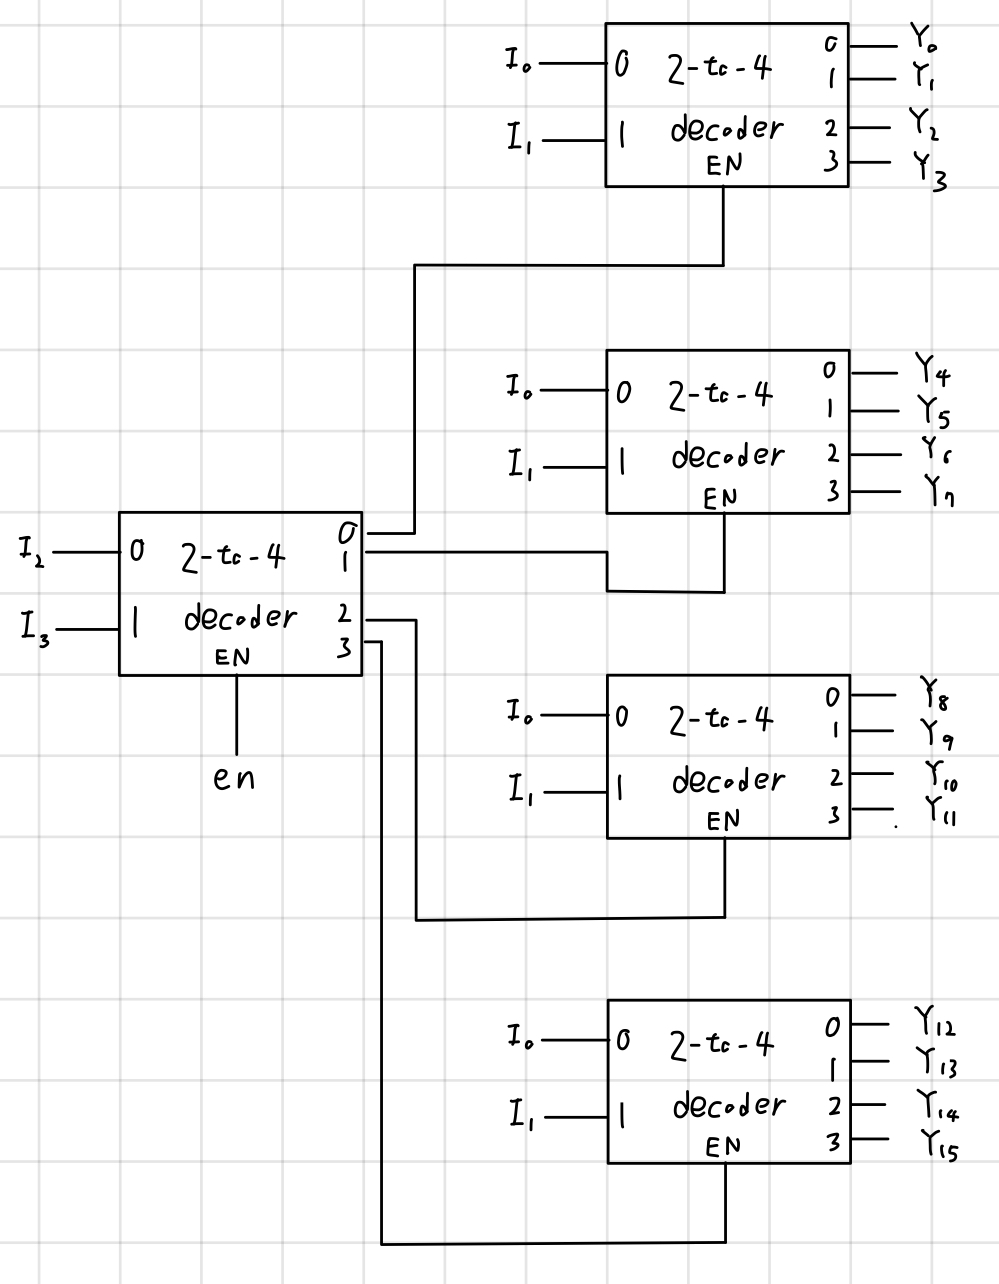
\includegraphics[width=0.7\linewidth]{decoder_expansion}
\end{figure}

\subsection{4-bit 소수 판별기}
4-bit 소수 판별기는 minterm 표기법으로 나타내면 다음과 같다.
\[
  F(A_0, A_1, A_2, A_3) = \sum m(0100_2, 1010_2, 1100_2, 1101_2, 1110_2)
\]
Truth table을 그리면
\begin{table}[H]
  \centering
  \begin{tabular}{|cccc|c|}
    \hline
    \(A_0\) & \(A_1\) & \(A_2\) & \(A_3\) & Out \\
    \hline
    0       & 0       & 0       & 0       & 0   \\
    0       & 0       & 0       & 1       & 0   \\
    0       & 0       & 1       & 0       & 0   \\
    0       & 0       & 1       & 1       & 0   \\
    0       & 1       & 0       & 0       & 1   \\
    0       & 1       & 0       & 1       & 0   \\
    0       & 1       & 1       & 0       & 0   \\
    0       & 1       & 1       & 1       & 0   \\
    1       & 0       & 0       & 0       & 0   \\
    1       & 0       & 0       & 1       & 0   \\
    1       & 0       & 1       & 0       & 1   \\
    1       & 0       & 1       & 1       & 0   \\
    1       & 1       & 0       & 0       & 1   \\
    1       & 1       & 0       & 1       & 1   \\
    1       & 1       & 1       & 0       & 1   \\
    1       & 1       & 1       & 1       & 0   \\
    \hline
  \end{tabular}
\end{table}
K-map을 그리면 다음과 같다.
\begin{figure}[H]
  \centering
  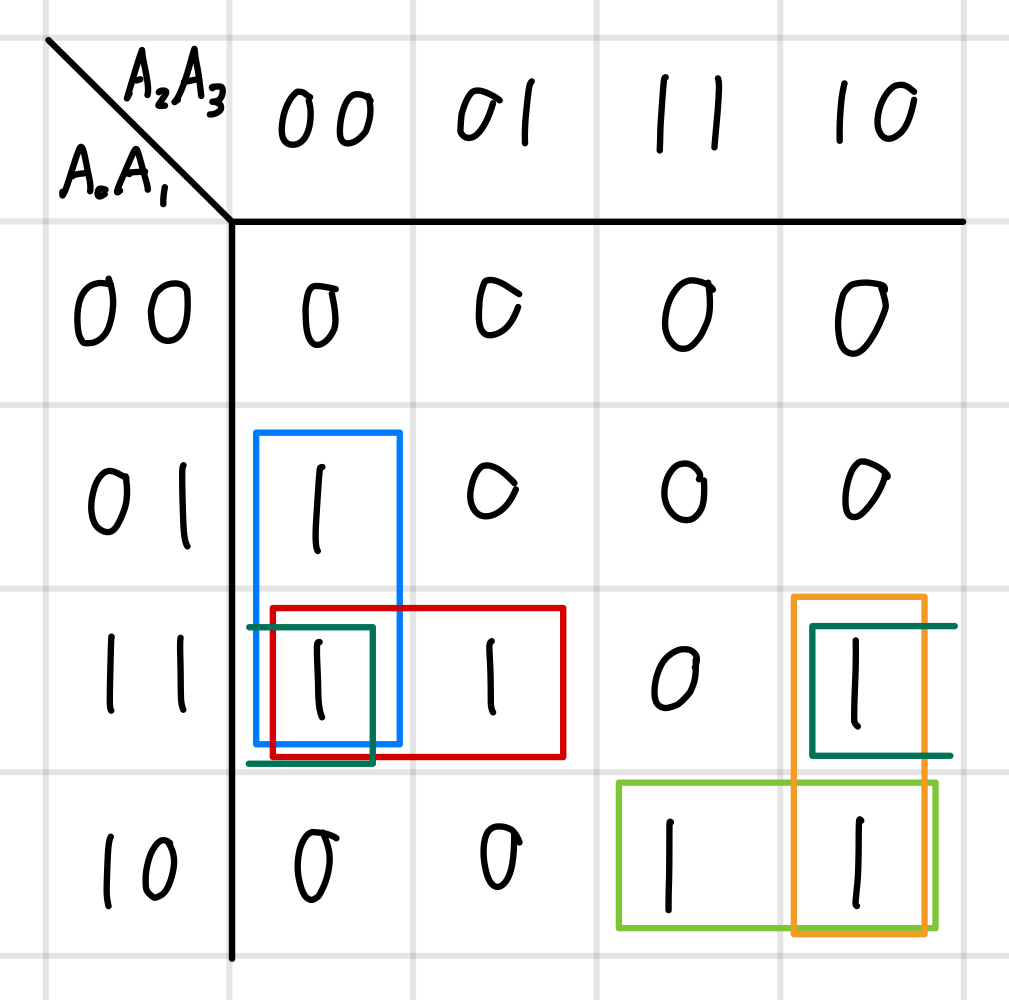
\includegraphics[width=0.3\linewidth]{lab3_2_km}
\end{figure}
EPI를 고르면 모든 1이 커버되므로, simplification한 대수식은 다음과 같다.
\[
  F(A_0, A_1, A_2, A_3) = A_0 A_1 A_2' + A_0 A_2 A_3' + A_1 A_2' A_3'
\]

\subsection{4-bit 배수 판별기}
11의 배수는 0, 11이므로, K-map을 그리면
\begin{figure}[H]
  \centering
  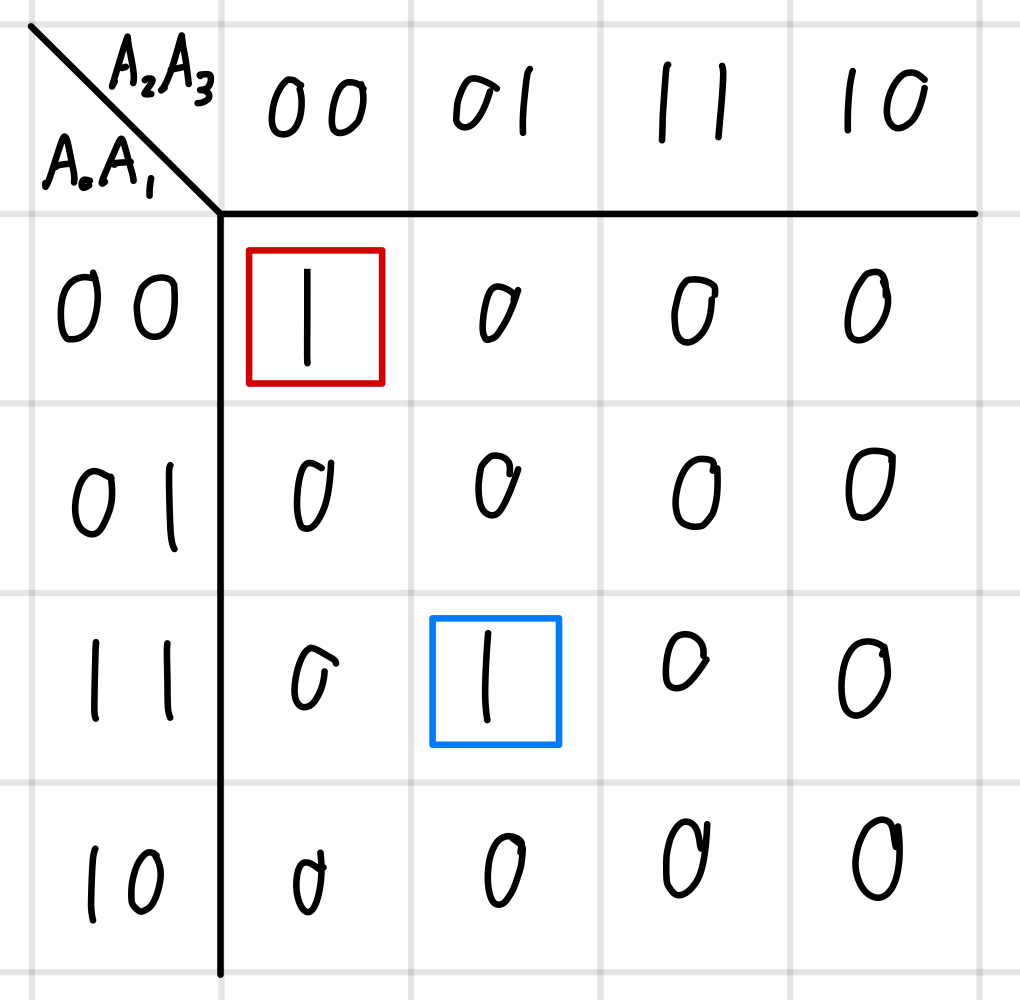
\includegraphics[width=0.3\linewidth]{lab3_2_11_km}
\end{figure}
따라서 simplification 한 결과는 다음과 같다.
\[
  F_{11}(A_0, A_1, A_2, A_3) = A_0' A_1' A_2' A_3' + A_0 A_1 A_2' A_3
\]

7의 배수는 0, 7, 14이므로, K-map을 그리면
\begin{figure}[H]
  \centering
  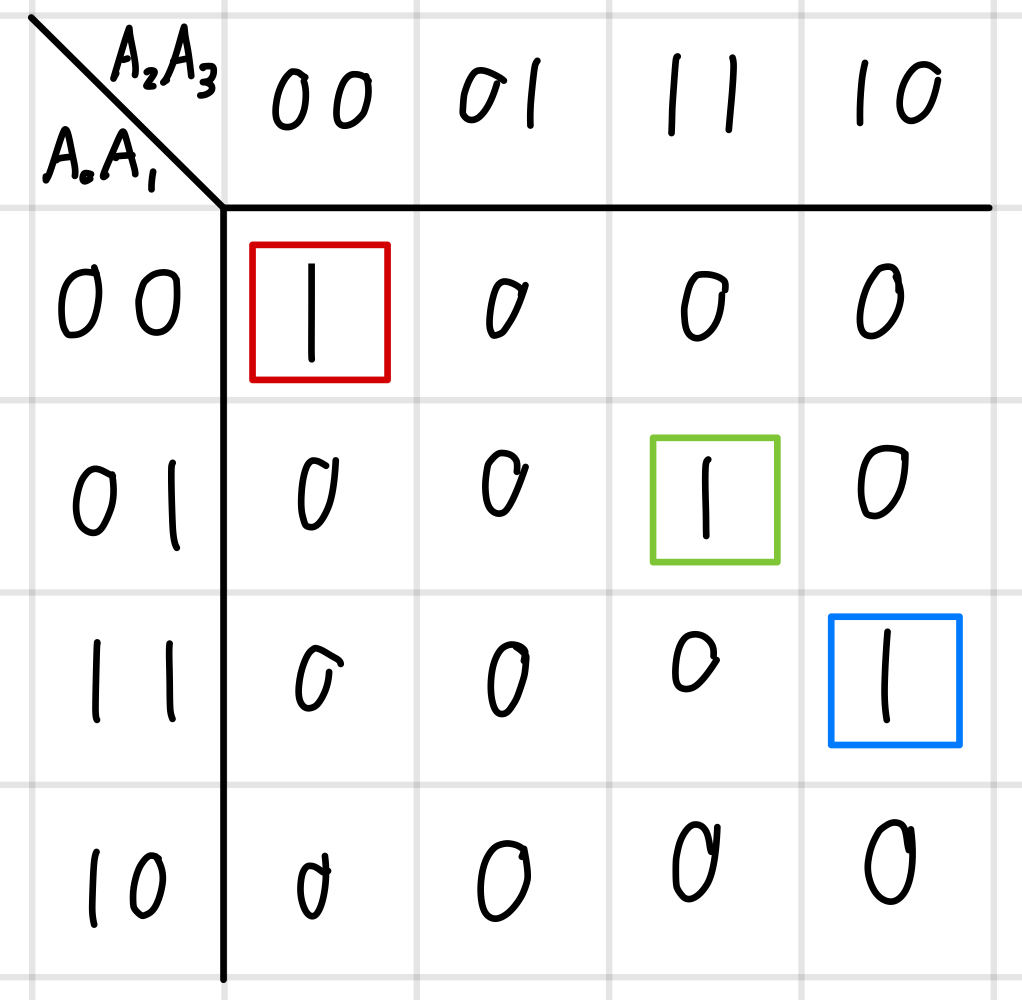
\includegraphics[width=0.3\linewidth]{lab3_2_7_km}
\end{figure}
따라서 simplification 한 결과는 다음과 같다.
\[
  F_7(A_0, A_1, A_2, A_3) = A_0' A_1' A_2' A_3' + A_0 A_1 A_2 A_3' + A_0' A_1 A_2 A_3
\]

5의 배수는 0, 5, 10, 15이므로, K-map을 그리면
\begin{figure}[H]
  \centering
  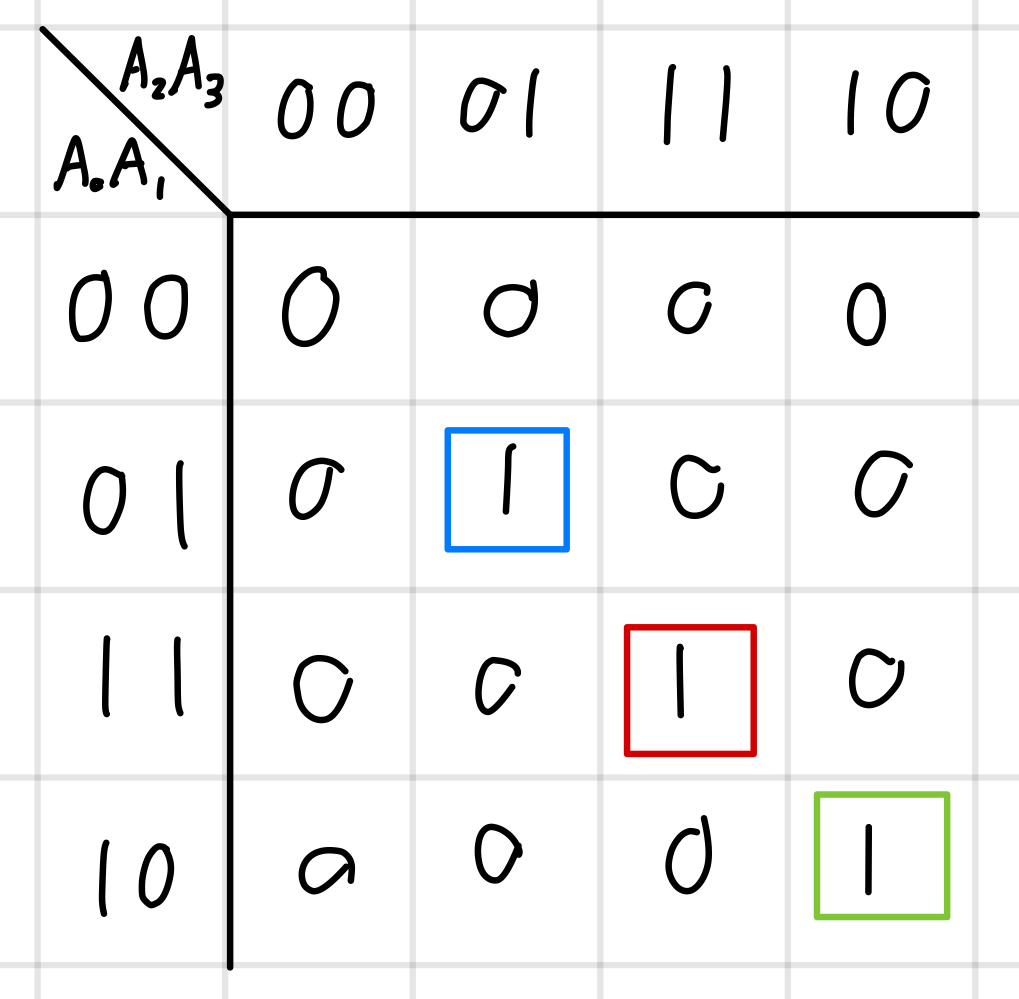
\includegraphics[width=0.3\linewidth]{lab3_2_5_km}
\end{figure}
따라서 simplification 한 결과는 다음과 같다.
\[
  F_5(A_0, A_1, A_2, A_3) = A_0' A_1' A_2' A_3' + A_0 A_1' A_2 A_3' + A_0' A_1 A_2' A_3 + A_0 A_1 A_2 A_3
\]

3의 배수는 0, 3, 6, 9, 12, 15이므로, K-map을 그리면
\begin{figure}[H]
  \centering
  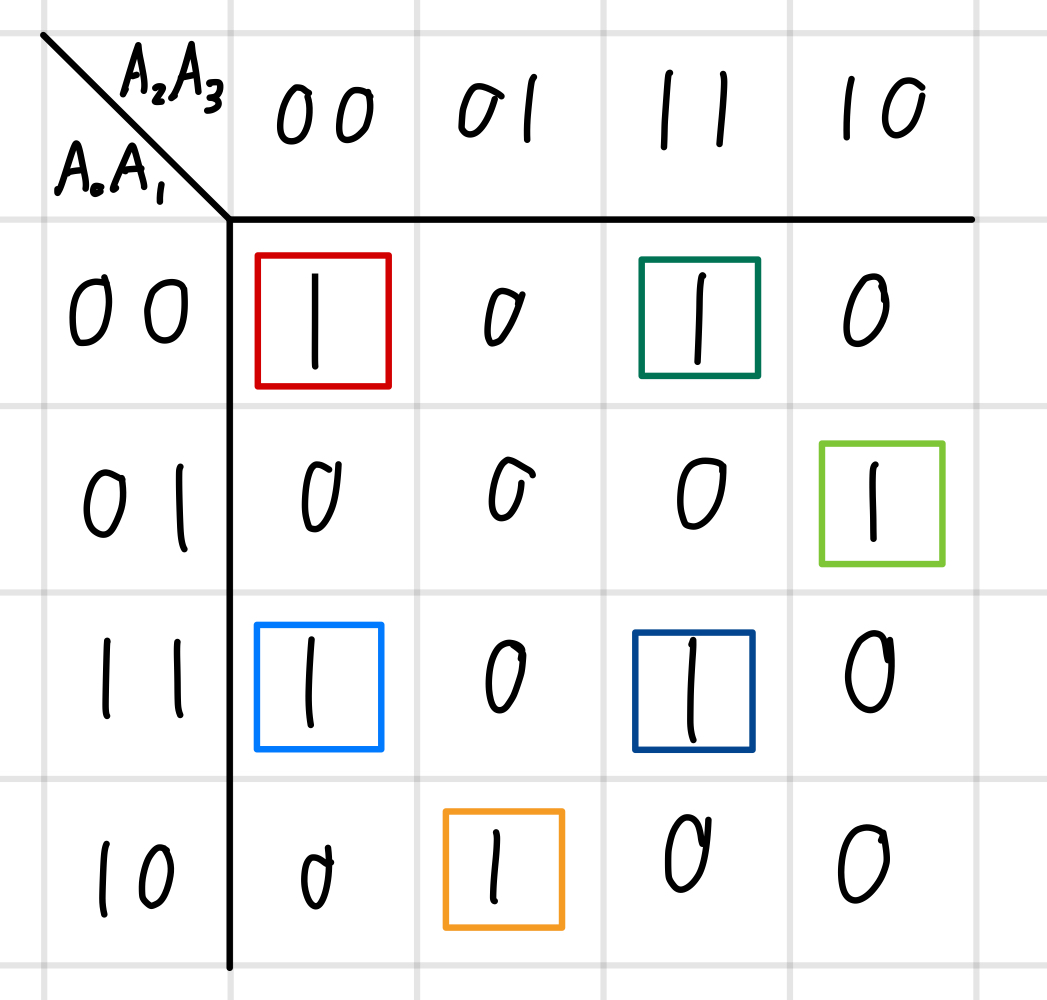
\includegraphics[width=0.3\linewidth]{lab3_2_3_km}
\end{figure}
따라서 simplification 한 결과는 다음과 같다.
\begin{align*}
  F_3(A_0, A_1, A_2, A_3) &= A_0' A_1' A_2' A_3' + A_0 A_1' A_2 A_3' + A_0' A_1 A_2' A_3 \\
                          &= A_0 A_1' A_2' A_3 + A_0' A_1' A_2 A_3 + A_0 A_1 A_2 A_3
\end{align*}

2의 배수는 0, 2, 4, 6, 8, 10, 12, 14이므로, K-map을 그리면
\begin{figure}[H]
  \centering
  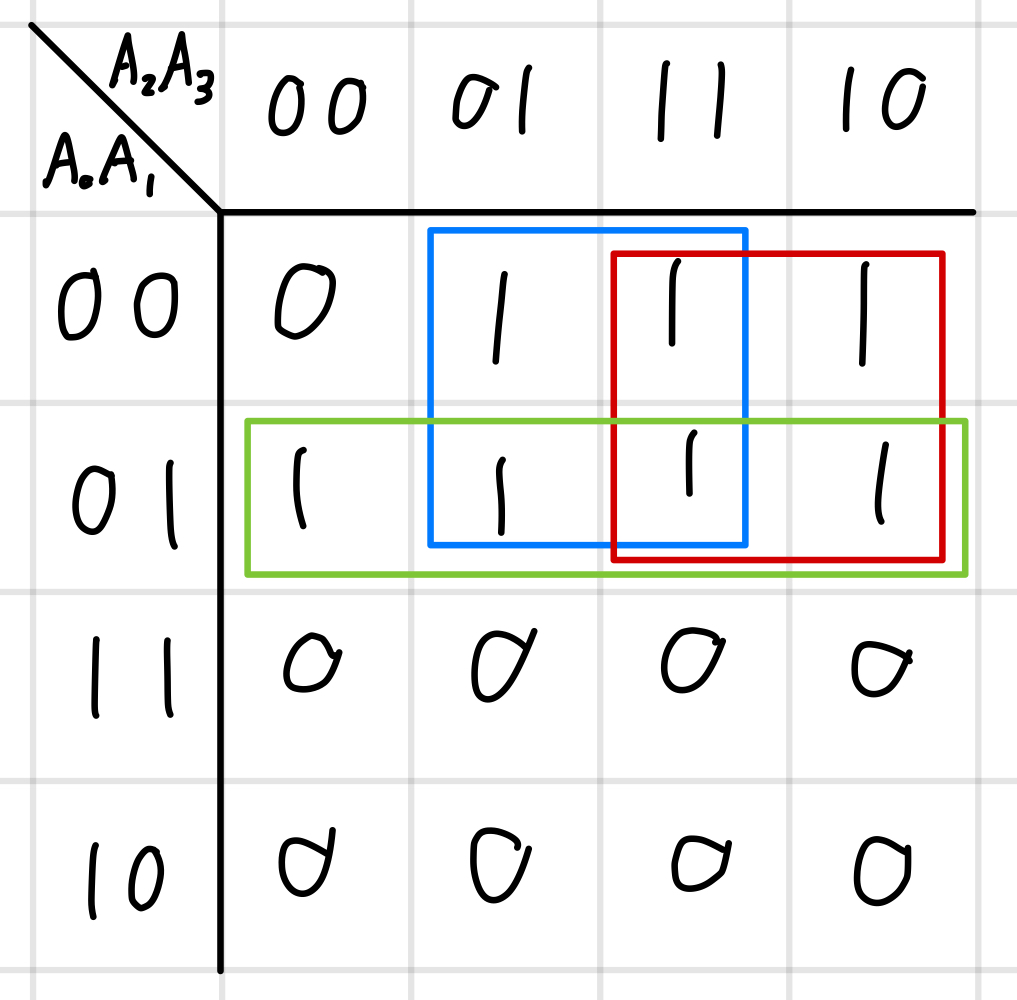
\includegraphics[width=0.3\linewidth]{lab3_2_2_km}
\end{figure}
따라서 simplification 한 결과는 다음과 같다.
\begin{align*}
  F_2(A_0, A_1, A_2, A_3) = A_0'
\end{align*}

\subsection{5-bit Majority Function}
5-bit majority function의 truth table은 다음과 같다.
\begin{table}[H]
  \centering
  \begin{tabular}{|ccccc|c|}
  \hline
  \(A\) & \(B\) & \(C\) & \(D\) & \(E\) & Out \\
  \hline
  0 & 0 & 0 & 0 & 0 & 0   \\
  0 & 0 & 0 & 0 & 1 & 0   \\
  0 & 0 & 0 & 1 & 0 & 0   \\
  0 & 0 & 0 & 1 & 1 & 0   \\
  0 & 0 & 1 & 0 & 0 & 0   \\
  0 & 0 & 1 & 0 & 1 & 0   \\
  0 & 0 & 1 & 1 & 0 & 0   \\
  0 & 0 & 1 & 1 & 1 & 1   \\
  0 & 1 & 0 & 0 & 0 & 0   \\
  0 & 1 & 0 & 0 & 1 & 0   \\
  0 & 1 & 0 & 1 & 0 & 0   \\
  0 & 1 & 0 & 1 & 1 & 1   \\
  0 & 1 & 1 & 0 & 0 & 0   \\
  0 & 1 & 1 & 0 & 1 & 1   \\
  0 & 1 & 1 & 1 & 0 & 1   \\
  0 & 1 & 1 & 1 & 1 & 1   \\
  1 & 0 & 0 & 0 & 0 & 0   \\
  1 & 0 & 0 & 0 & 1 & 0   \\
  1 & 0 & 0 & 1 & 0 & 0   \\
  1 & 0 & 0 & 1 & 1 & 1   \\
  1 & 0 & 1 & 0 & 0 & 0   \\
  1 & 0 & 1 & 0 & 1 & 1   \\
  1 & 0 & 1 & 1 & 0 & 1   \\
  1 & 0 & 1 & 1 & 1 & 1   \\
  1 & 1 & 0 & 0 & 0 & 0   \\
  1 & 1 & 0 & 0 & 1 & 1   \\
  1 & 1 & 0 & 1 & 0 & 1   \\
  1 & 1 & 0 & 1 & 1 & 1   \\
  1 & 1 & 1 & 0 & 0 & 1   \\
  1 & 1 & 1 & 0 & 1 & 1   \\
  1 & 1 & 1 & 1 & 0 & 1   \\
  1 & 1 & 1 & 1 & 1 & 1   \\
  \hline
  \end{tabular}
\end{table}
SOP 형태로 바꾸면 다음과 같다.
\begin{align*}
  F(A, B, C, D, E) &= A' B' C D E + A' B C' D E + A' B C D' E \\
                   &+ A' B C D E' + A' B C D E + A B' C' D E \\
                   &+ A B' C D' E + A B' C D E' + A B' C D E \\
                   &+ A B C' D' E + A B C' D E' + A B C' D E \\
                   &+ A B C D' E' + A B C D' E + A B C D E' + A B C D E
\end{align*}
한편, 이를 정리하면
\begin{align*}
  F(A, B, C, D, E) &= AB (C' D' E + C' D E' + C D' E') \\
                   &+ (A + B)(C' D E + C D' E + C D E') + CDE \\
\end{align*}
멀티플렉서의 선택 신호를 \(C, D, E\)로 하고, 입력 신호를 \(0, 1, AB, A + B\) 중에서 적절히 고르면 \(F\)를 구현할 수 있을 것이다.
이를 나타내면 다음과 같다.
\begin{table}[H]
  \centering
  \begin{tabular}{|ccc|l|}
  \hline
  \(C\) & \(D\) & \(E\) & Input \\
  \hline
  0 & 0 & 0 & 0 \\
  0 & 0 & 1 & \(AB\) \\
  0 & 1 & 0 & \(AB\) \\
  0 & 1 & 1 & \(A + B\) \\
  1 & 0 & 0 & \(AB\) \\
  1 & 0 & 1 & \(A + B\) \\
  1 & 1 & 0 & \(A + B\) \\
  1 & 1 & 1 & 1 \\
  \hline
  \end{tabular}
\end{table}

\section{실험 결과}
\texttt{lab3\_1.v}의 테스트벤치를 실행하여 얻은 결과는 다음과 같다.
\begin{figure}[H]
  \centering
  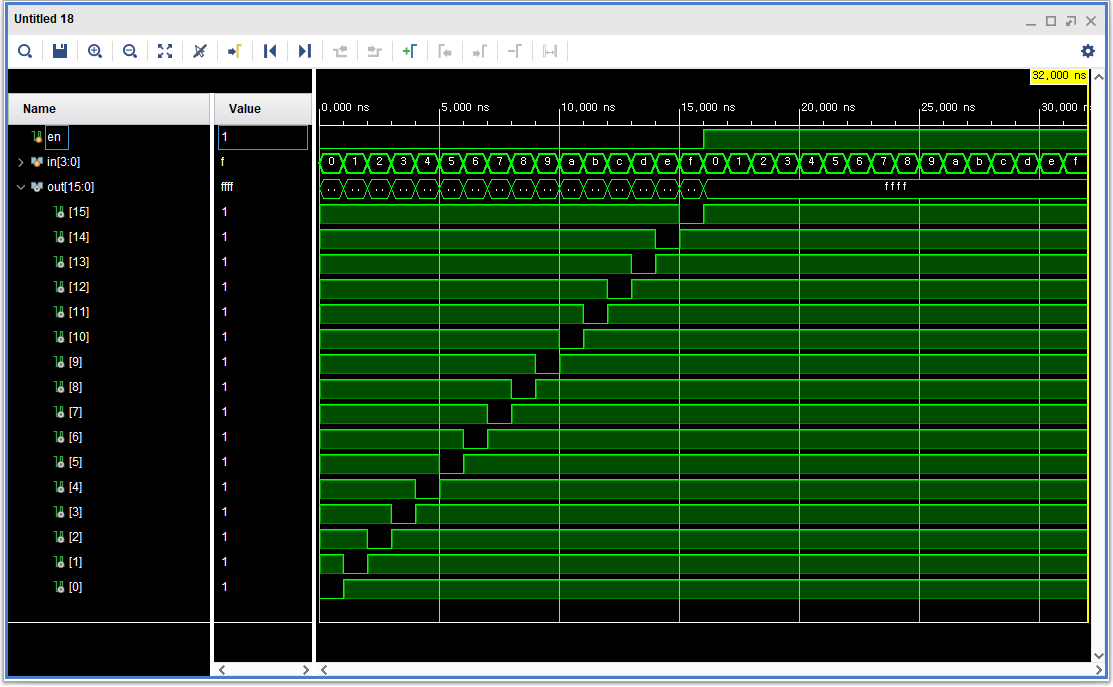
\includegraphics[width=\linewidth]{lab3_1_waveform}
\end{figure}
입력으로 들어가는 4비트 숫자가 1씩 증가하면서 `참'에 해당하는 출력이 한 개의 핀에서만 나오는 것을 볼 수 있고, \texttt{en}이 1일때, 즉 비활성화 상태에서는 모든 출력 핀에서 `거짓'에 해당되는 출력이 나오는 것을 볼 수 있었다.
다음과 같은 schematic을 얻을 수 있었다.
\begin{figure}[H]
  \centering
  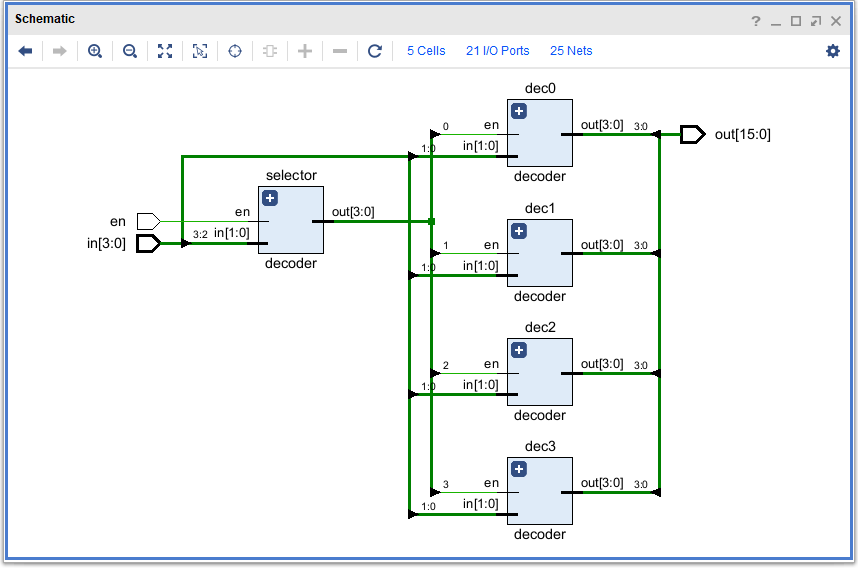
\includegraphics[width=\linewidth]{lab3_1_schematic}
\end{figure}

\texttt{lab3\_2.v}의 테스트벤치 실행 결과는 다음과 같다.
\begin{figure}[H]
  \centering
  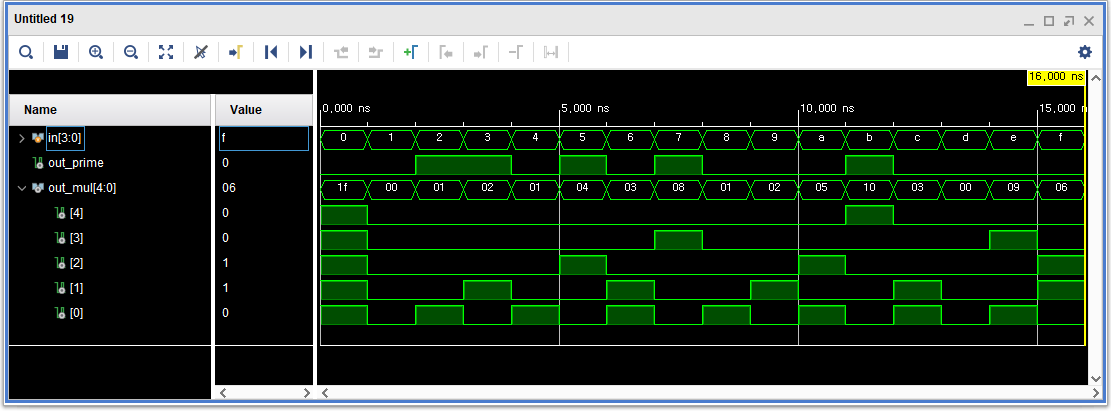
\includegraphics[width=\linewidth]{lab3_2_waveform}
\end{figure}
2, 3, 5, 7, 11에 대해 \texttt{out\_prime}에서 소수 판정 결과를 1로 나타내는 것을 볼 수 있다.
배수 판정의 경우, MSB부터 11, 7, 5, 3, 2의 배수인지에 대한 결과가 정확하게 나타남을 볼 수 있다.
Schematic은 다음과 같다.
\begin{figure}[H]
  \centering
  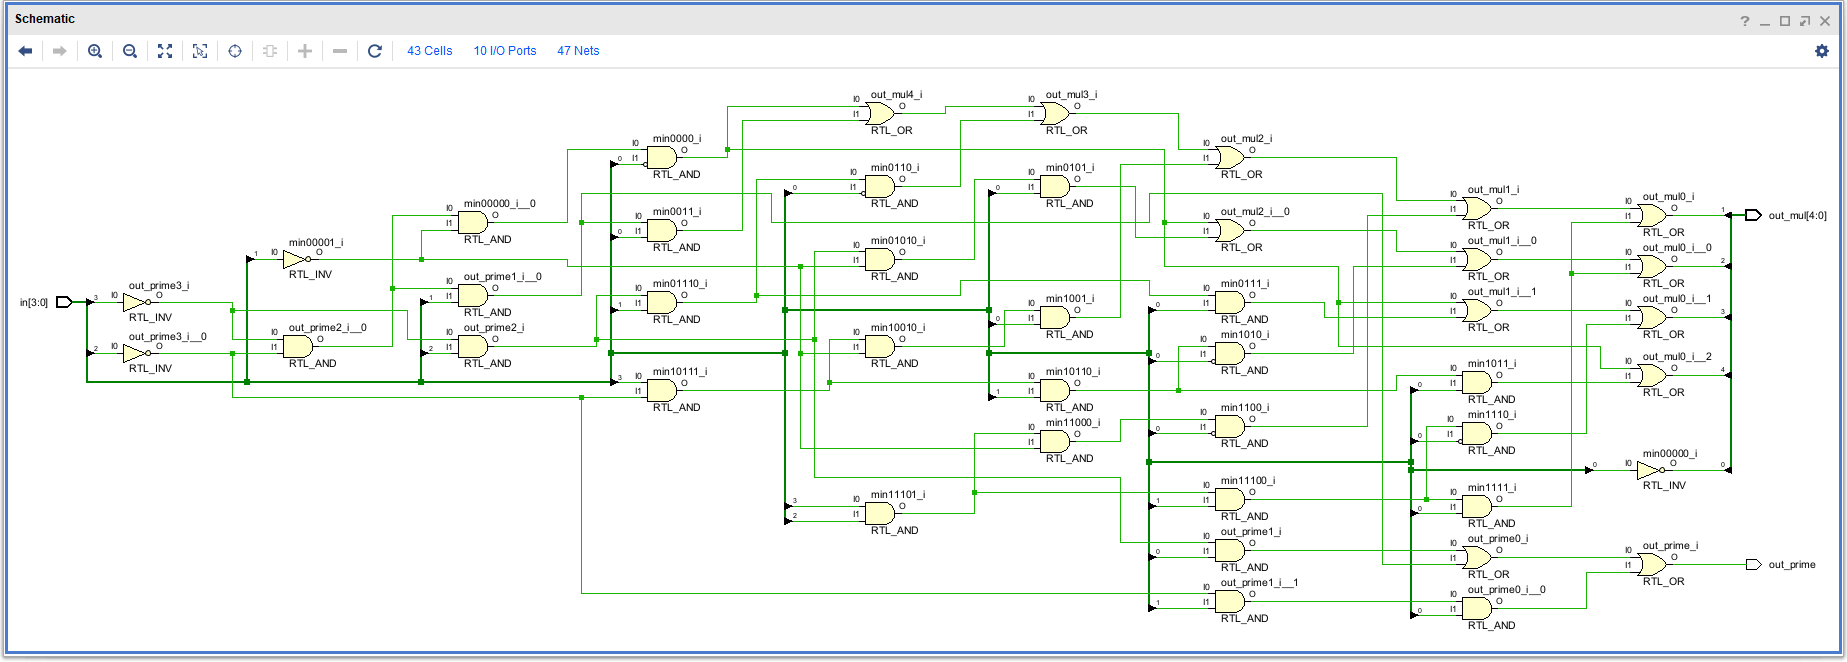
\includegraphics[width=\linewidth]{lab3_2_schematic}
\end{figure}

\texttt{lab3\_3.v}의 테스트벤치 실행 결과는 다음과 같다.
\begin{figure}[H]
  \centering
  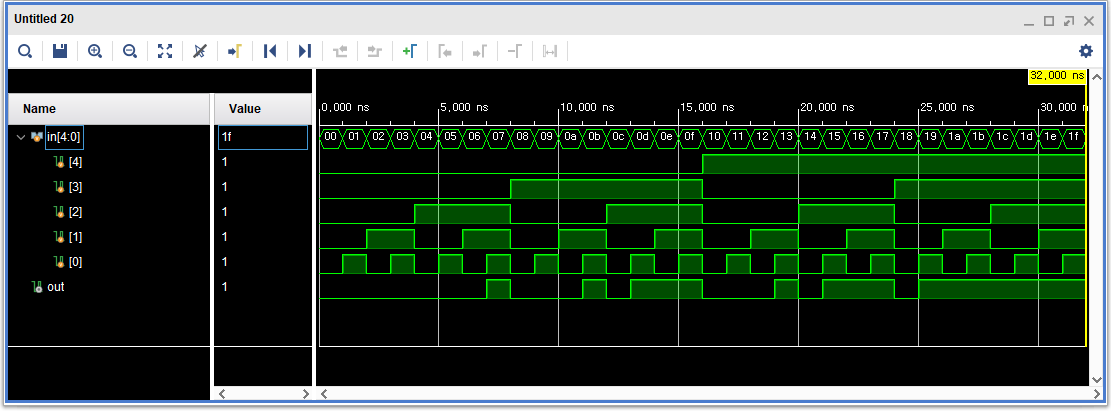
\includegraphics[width=\linewidth]{lab3_3_waveform}
\end{figure}
0과 1 중에서 더 개수가 많은 수를 정확히 출력함을 볼 수 있다.
Schematic은 다음과 같다.
\begin{figure}[H]
  \centering
  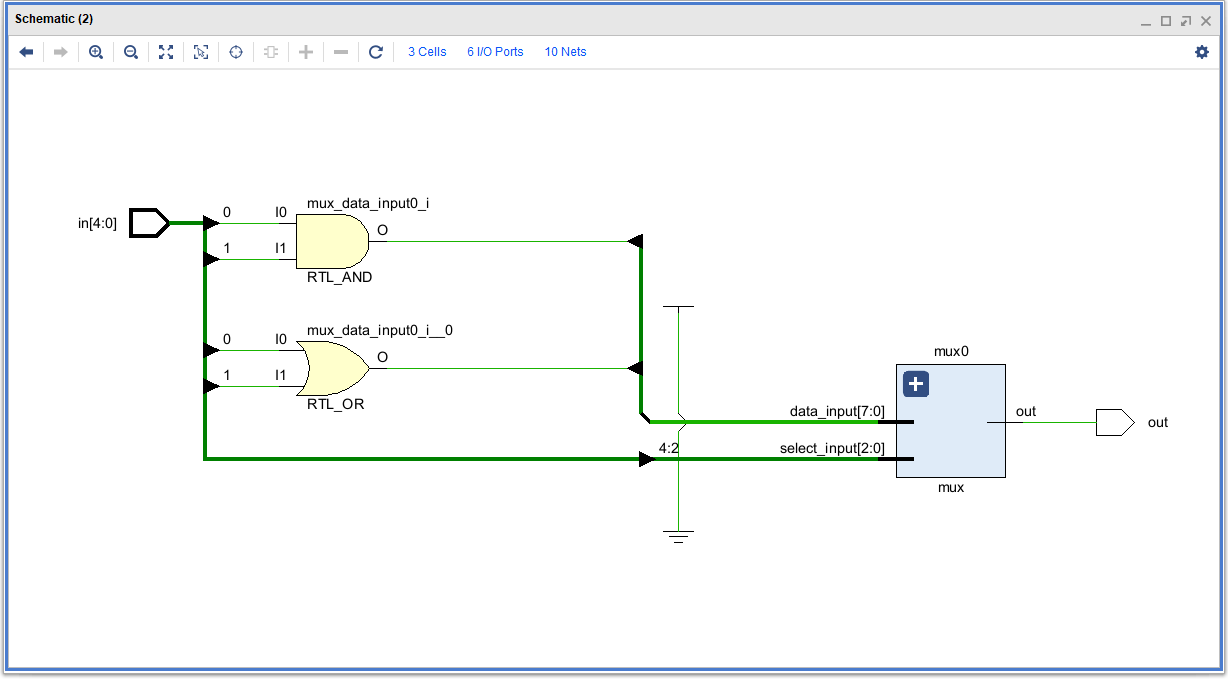
\includegraphics[width=\linewidth]{lab3_3_schematic}
\end{figure}

\section{논의}
이번 lab 3에서는 디코더와 멀티플렉서를 사용하여 다른 소자를 구현해 볼 수 있었다.
수업 시간에 이론으로 들었던 내용이 실제 적용되는 모습을 볼 수 있어서 이들 소자를 이해하는 데에 도움이 되었다.

\end{document}
